\documentclass[UTF8,a4paper,11pt]{ctexart}

\usepackage{geometry}
\usepackage{graphicx}
\usepackage{hyperref}
\usepackage{booktabs}
\usepackage{listings}
\usepackage{xcolor}
\usepackage{caption}
\usepackage{subcaption}
\usepackage{enumitem}

\geometry{left=2.5cm,right=2.5cm,top=2.8cm,bottom=2.8cm}

\hypersetup{
  colorlinks=true,
  linkcolor=blue!60!black,
  urlcolor=cyan!40!black,
  citecolor=green!40!black
}

\lstset{
  basicstyle=\ttfamily\small,
  keywordstyle=\color{blue},
  commentstyle=\color{gray},
  breaklines=true,
  frame=single,
  backgroundcolor=\color{gray!8}
}

\title{\textbf{异构无人机集群灯光秀模拟软件开发日志}}
\author{朱华天 \and Claude Fable 5 \and Grok 4.5 \and Composer 2.5}
\date{2026年7月21日}

\begin{document}
\maketitle

\begin{abstract}
本文记录 \textbf{SWARM COMMAND} 异构无人机集群灯光秀模拟软件的开发过程。系统基于 TypeScript 与 Three.js 构建三维可视化与工业风控制台，采用三维 ORCA（Optimal Reciprocal Collision Avoidance）算法实现 200 架规模异构机群的实时避障与编队飞行，并通过 Tauri 2 打包为轻量化 Windows 桌面应用。全文涵盖需求分析、架构设计、核心模块实现、界面演进、性能优化与桌面发布等环节。
\end{abstract}

\tableofcontents
\newpage

\section{项目概述}

\subsection{背景与动机}
无人机集群灯光秀已成为城市夜景与大型活动的重要组成部分。与传统均质编队不同，\emph{异构集群}——由侦察、运输、中继等多类型机型协同——更贴近真实工业场景，但也带来差异化的动力学约束与避障责任分配问题。本项目旨在开发一款兼具\textbf{电影感演示}与\textbf{工业级监控}能力的桌面仿真软件，为集群算法验证与视觉方案预演提供工具。

\subsection{设计目标}
\begin{itemize}[leftmargin=2em]
  \item 支持 100--300 架无人机实时仿真，目标帧率 60\,FPS；
  \item 三种异构机型：侦察四旋翼（快/小）、运输六旋翼（大/慢/高优先级）、通信中继机（稳/中）；
  \item 三维 ORCA 互惠避障，保证机间无碰撞；
  \item 七种队形切换：地面阵列、球面警戒、双螺旋、分层环形、楔形突击、星爆散开、灯光文字；
  \item 电影感渲染：Bloom 辉光、夜景氛围、自动导演运镜；
  \item 工业风控制台：遥测面板、任务规划、告警流、故障演练；
  \item 通过 Tauri 2 打包为轻量化 Windows 可执行程序。
\end{itemize}

\section{技术架构}

系统采用四层架构，仿真内核与渲染层解耦，便于独立测试与后续扩展。

\begin{description}[leftmargin=3em,style=nextline]
  \item[仿真内核] \texttt{src/core/}：Vec3 向量、空间哈希、ORCA 求解器、无人机实体、集群管理、队形生成。
  \item[渲染层] \texttt{src/render/}：Three.js 场景、InstancedMesh 异构机型、飞行拖尾、后期特效、摄影导演。
  \item[控制台] \texttt{src/ui/}：顶栏状态、左右侧栏（任务/遥测/告警）、原生 CSS 工业 HUD 风格。
  \item[桌面壳] \texttt{src-tauri/}：Tauri 2 + WebView2，将前端静态资源嵌入原生窗口。
\end{description}

主循环采用\textbf{固定步长仿真}（$1/60$\,s）+ \textbf{可变帧率渲染}的经典游戏循环模式；UI 更新节流至约 8\,Hz，降低 DOM 开销。

\section{核心模块}

\subsection{三维 ORCA 避障}
ORCA 为每个近邻构造互惠速度障碍半平面，通过三维线性规划求解距离期望速度最近的可行速度。异构性通过以下参数体现：
\begin{itemize}[leftmargin=2em]
  \item \textbf{半径}：运输机 2.2\,m，侦察机 1.1\,m；
  \item \textbf{最大速度}：侦察 14\,m/s，运输 8\,m/s；
  \item \textbf{避让责任系数 yielding}：运输机 0.55（少让路），侦察机 1.4（多让路）。
\end{itemize}

近邻查询采用均匀网格空间哈希，每帧重建索引，查询时扫描 $3\times3\times3$ 单元，复杂度近似 $O(n)$。

\subsection{队形生成与目标分配}
七种队形由 \texttt{formations.ts} 生成目标点阵列。分层环形与楔形编队按机型分层：运输机居中/内层，中继机中环，侦察机外翼。目标分配采用贪心 2-opt 交换，在同机型内部降低交叉飞行距离。

\subsection{异构机型渲染}
每机型使用独立 \texttt{InstancedMesh}：机身（PBR 碳纤维材质）、实体桨叶、运动模糊桨盘、实例色航灯。200 架规模下 draw call 保持在个位数级。航灯配合 UnrealBloomPass 产生夜景辉光效果。

\subsection{摄影导演系统}
\texttt{cameraDirector.ts} 在自动模式下周期性切换五种机位：环绕、跟拍、掠过、俯瞰、升起仰拍。用户拖动画面时自动退出导演模式，切换为 OrbitControls 手动操控。

\section{界面演进}

初版采用 HUD 面板悬浮于三维场景之上，信息密度高但遮挡视口。根据使用反馈，第二版重构为\textbf{标准应用壳布局}：
\begin{itemize}[leftmargin=2em]
  \item 顶栏：品牌与机队总览指标；
  \item 左侧栏：任务规划与指挥控制；
  \item 中间视口：纯 3D 场景（仅保留左下角机位信息）；
  \item 右侧栏：机队构成、单机遥测、事件日志。
\end{itemize}

画布尺寸随中间视口自适应，点击拾取按视口坐标计算，避免侧栏挤压导致的交互偏差。

\section{界面截图}

\begin{figure}[htbp]
  \centering
  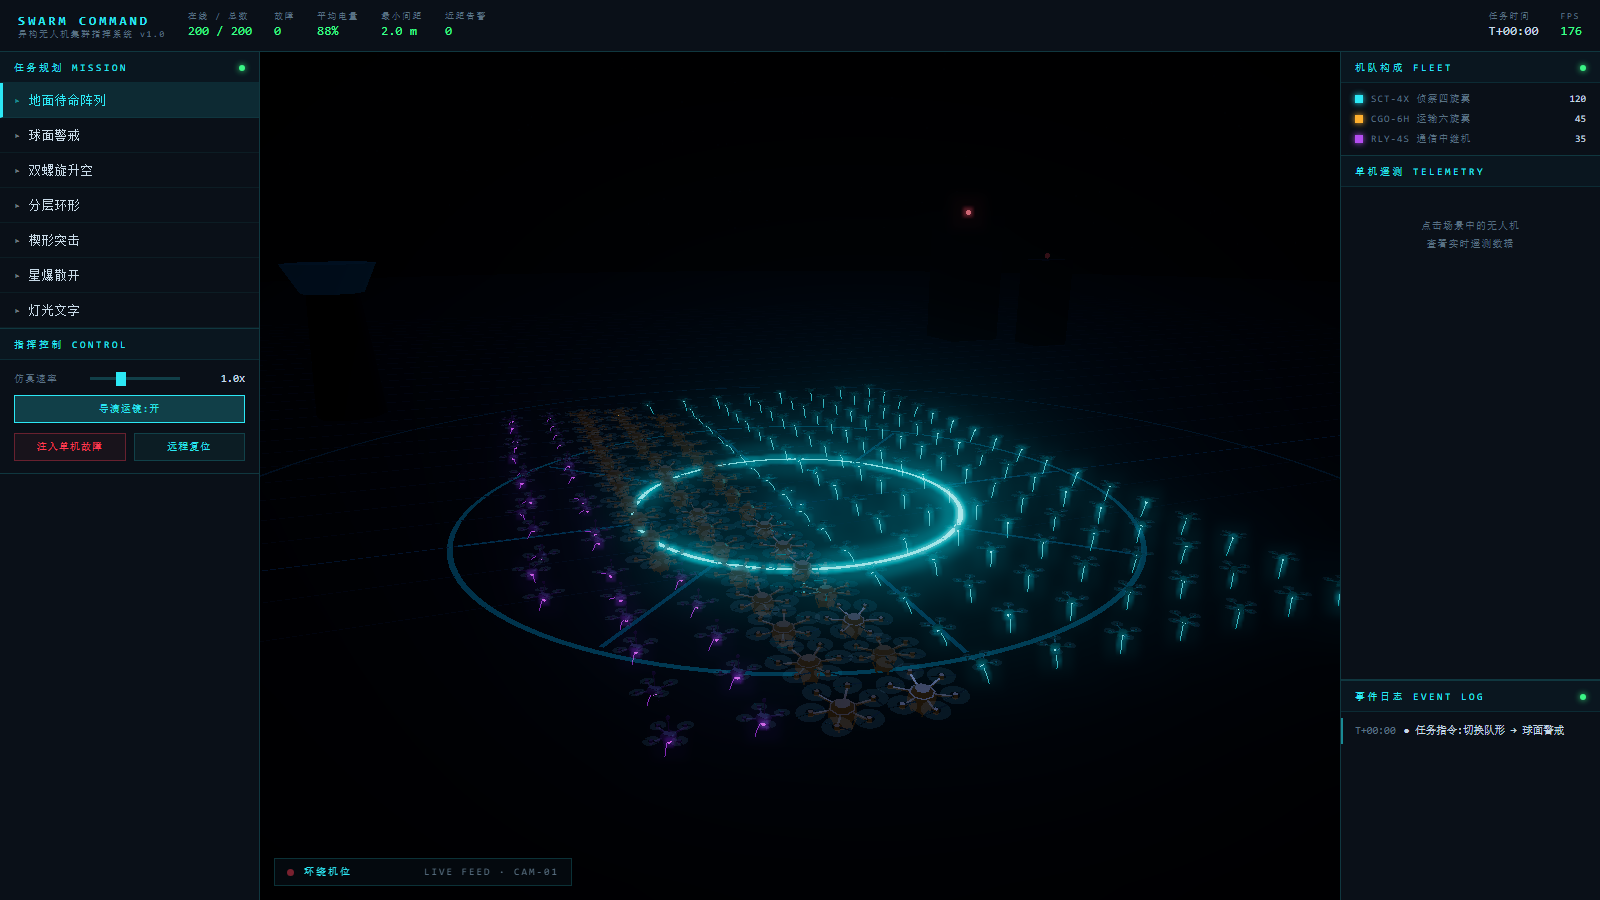
\includegraphics[width=0.92\textwidth]{screenshots/01-main-ui.png}
  \caption{侧栏布局总览：左任务、中视口、右遥测}
\end{figure}

\begin{figure}[htbp]
  \centering
  \begin{subfigure}{0.48\textwidth}
    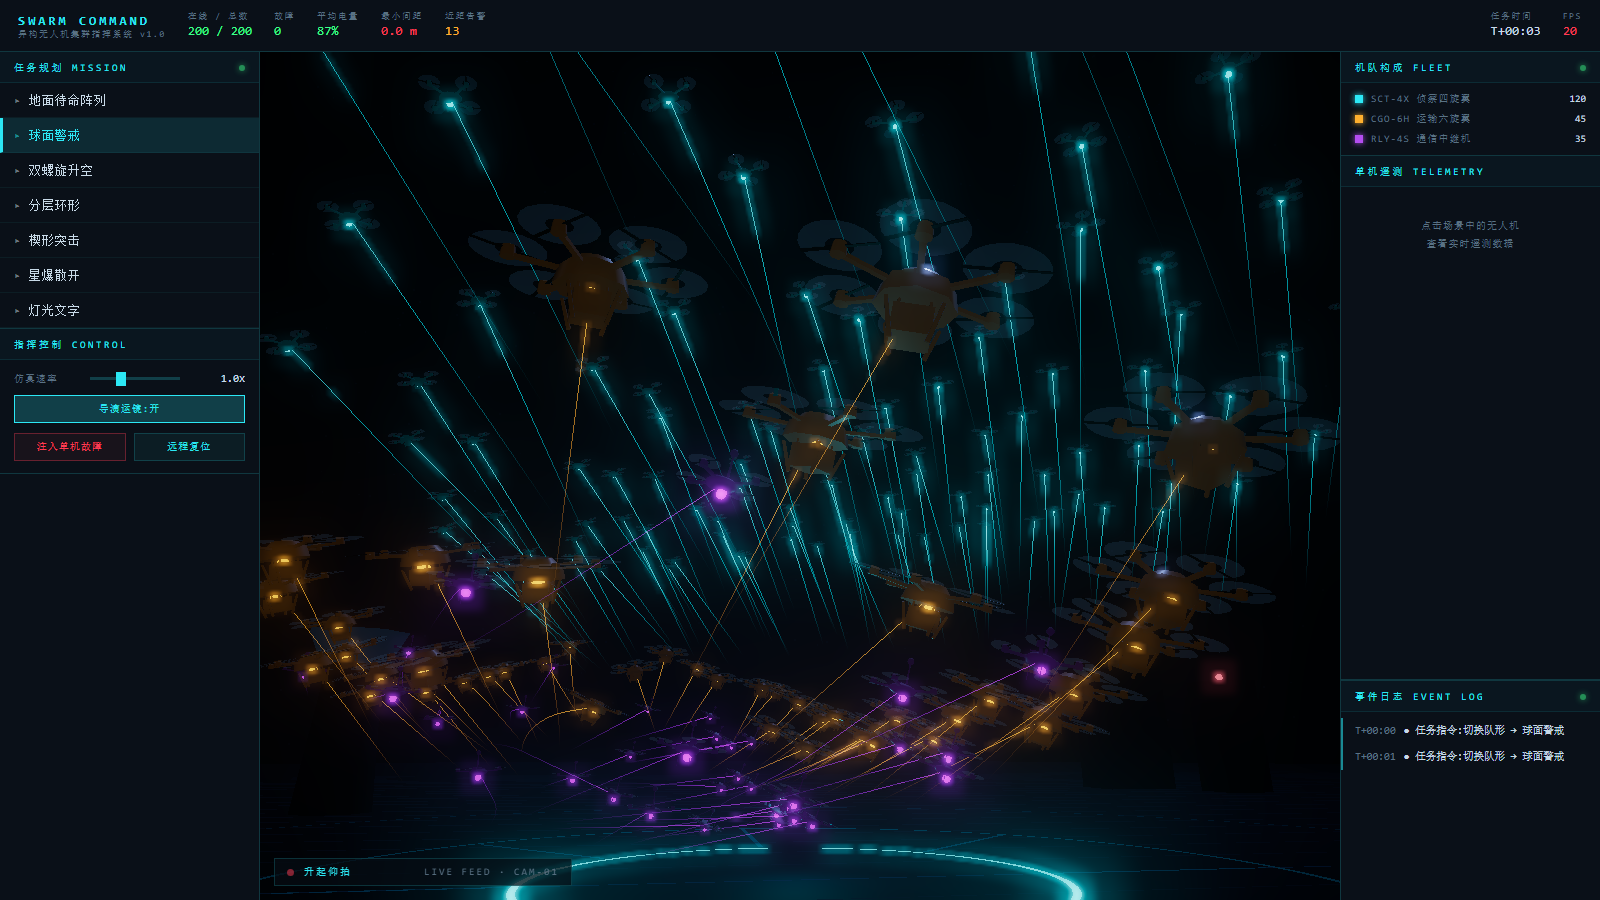
\includegraphics[width=\textwidth]{screenshots/02-sphere-formation.png}
    \caption{球面警戒队形}
  \end{subfigure}
  \hfill
  \begin{subfigure}{0.48\textwidth}
    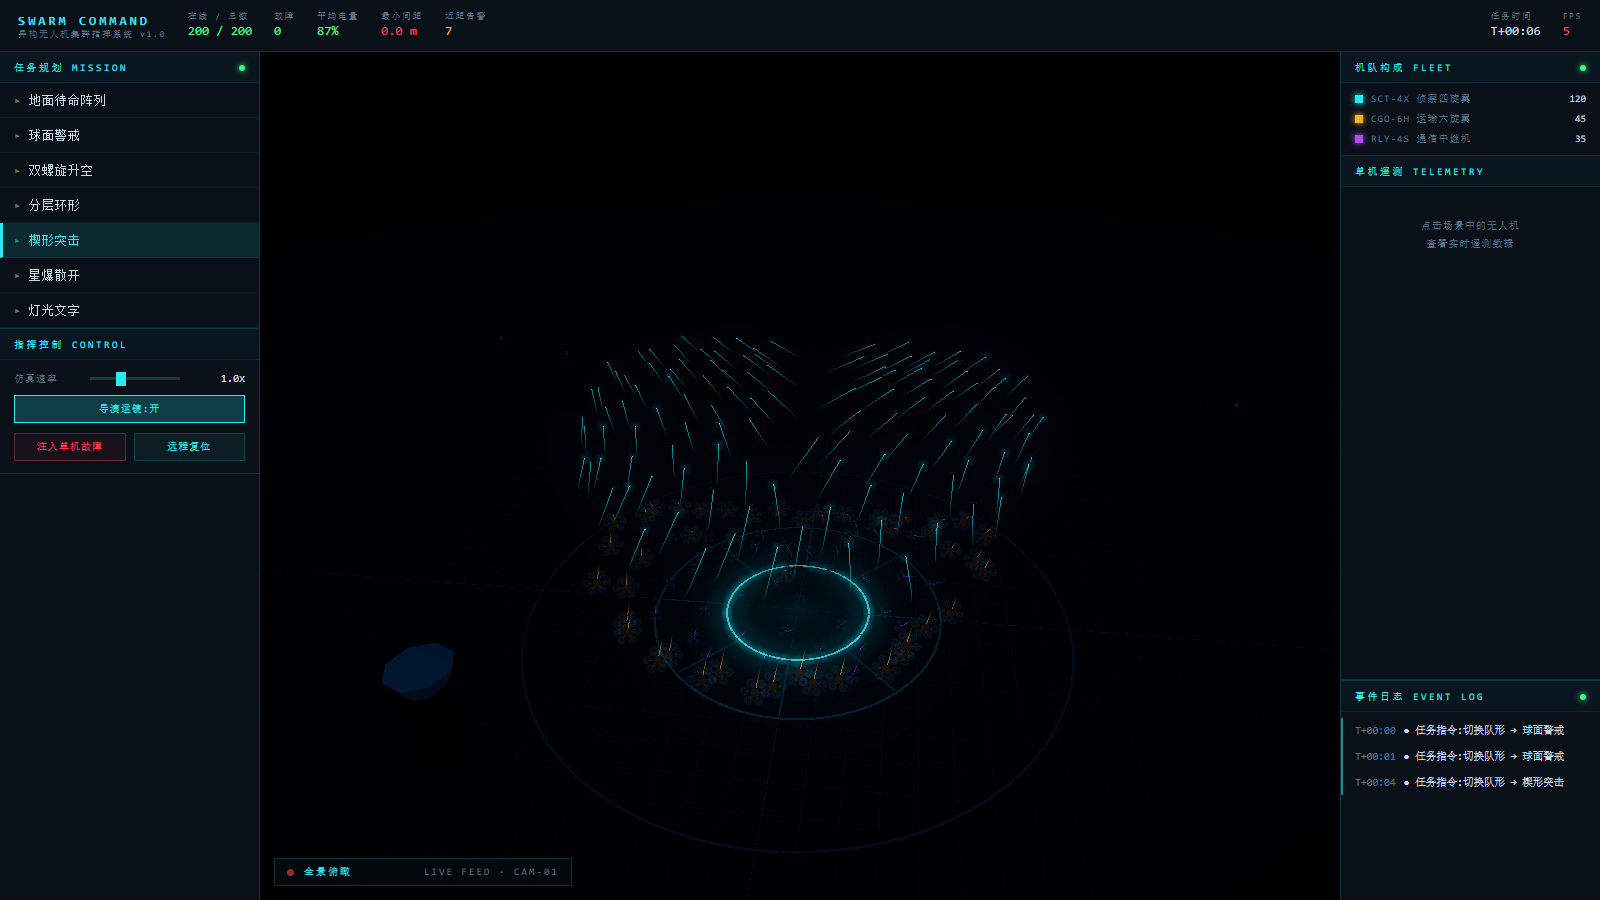
\includegraphics[width=\textwidth]{screenshots/03-phalanx-formation.png}
    \caption{楔形突击编队}
  \end{subfigure}
  \caption{两种典型队形切换效果}
\end{figure}

\begin{figure}[htbp]
  \centering
  \begin{subfigure}{0.48\textwidth}
    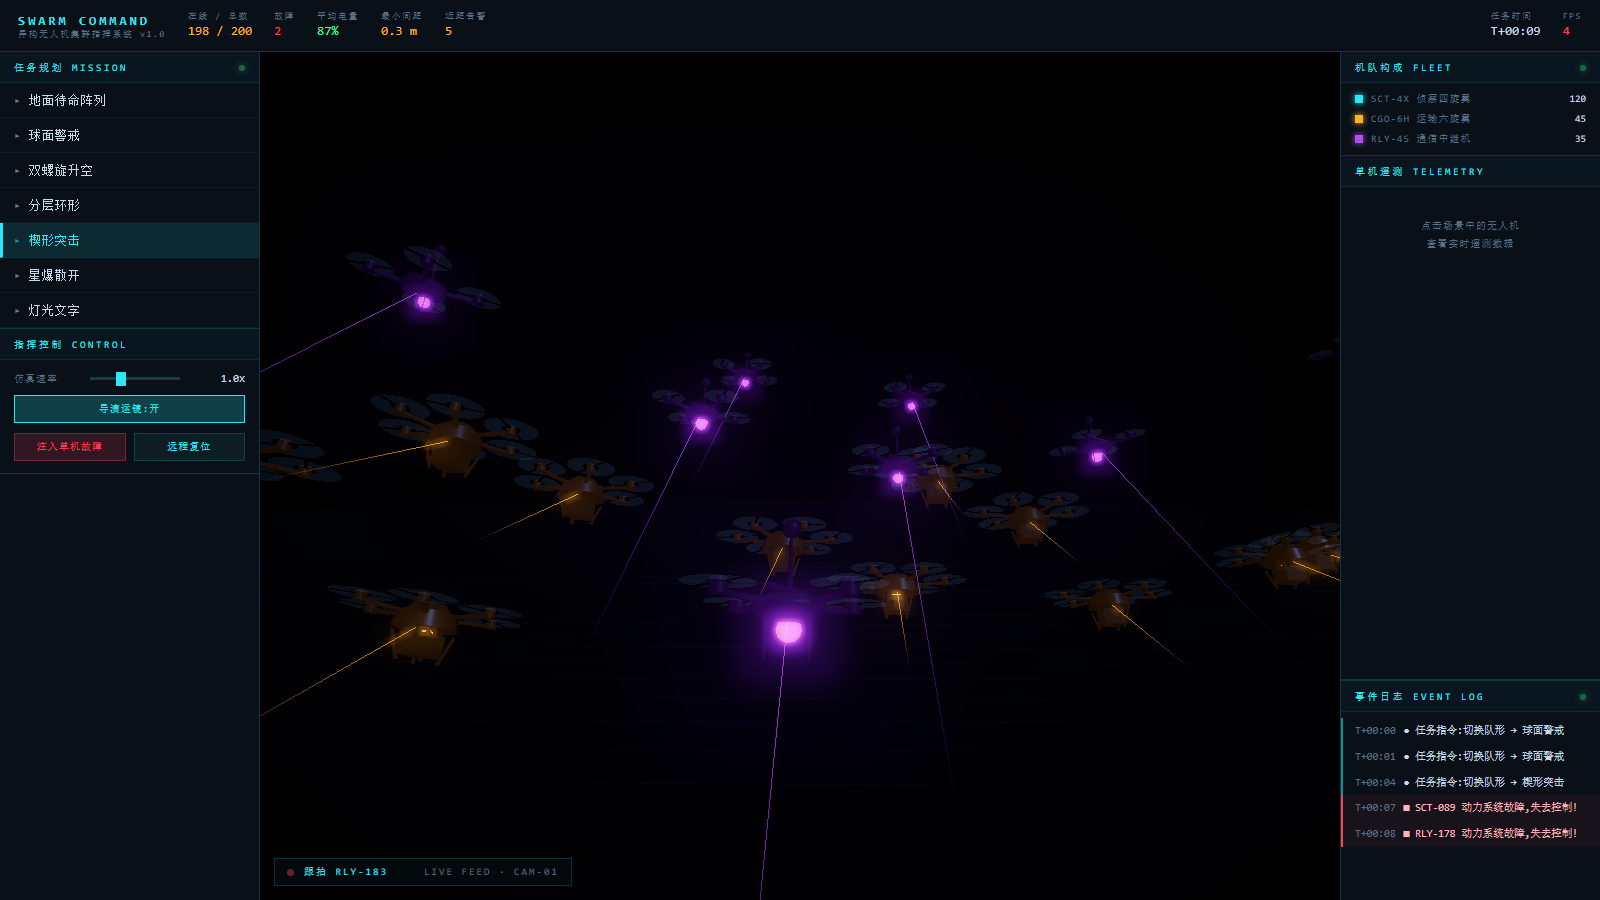
\includegraphics[width=\textwidth]{screenshots/04-failure-drill.png}
    \caption{单机故障演练与告警}
  \end{subfigure}
  \hfill
  \begin{subfigure}{0.48\textwidth}
    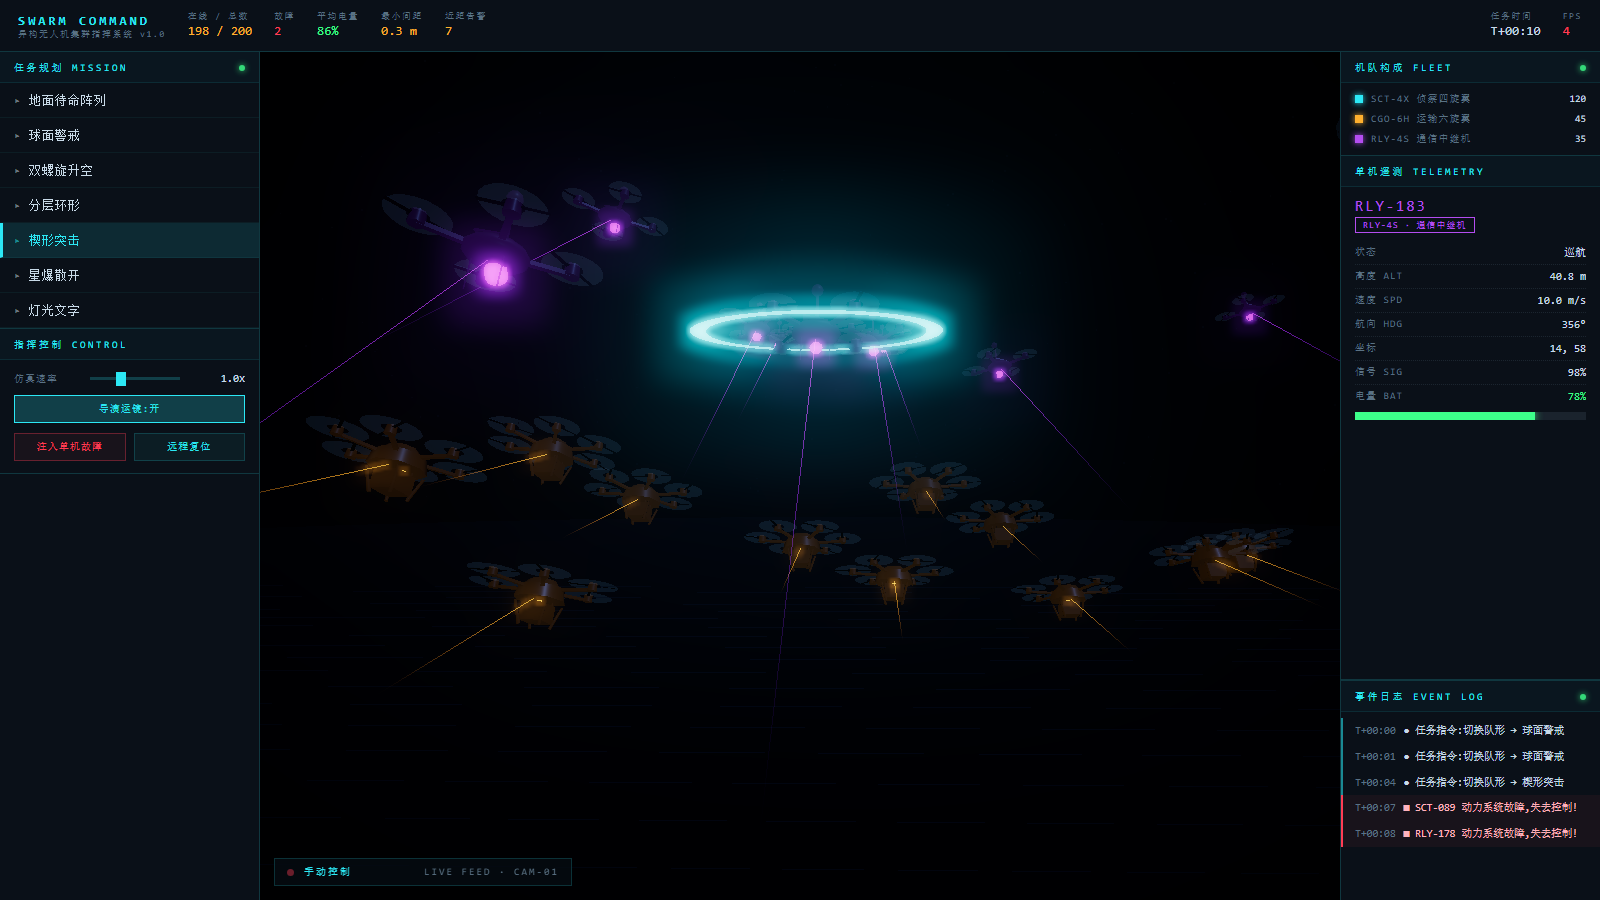
\includegraphics[width=\textwidth]{screenshots/05-telemetry.png}
    \caption{单机遥测面板}
  \end{subfigure}
  \caption{工业控制台功能展示}
\end{figure}

\section{性能与桌面打包}

\subsection{仿真性能}
在 200 架（120 侦察 + 45 运输 + 35 中继）配置下，ORCA 内核单步耗时约 1--3\,ms，主线程可稳定维持 60\,FPS。空间哈希将近邻候选从 $O(n^2)$ 降至近似线性。

\subsection{Tauri 2 轻量化配置}
为控制安装包体积，采用以下策略：
\begin{itemize}[leftmargin=2em]
  \item Rust \texttt{release}：\texttt{opt-level = "z"}、LTO、\texttt{strip = true}、\texttt{panic = "abort"}；
  \item Tauri 依赖：\texttt{default-features = false}，仅启用 \texttt{wry}；
  \item Windows 打包：NSIS + LZMA 压缩；
  \item 前端：Vite 生产构建 minify，\texttt{base: './'} 适配本地协议。
\end{itemize}

构建命令：
\begin{lstlisting}[language=bash]
npm install
npm run tauri:build
\end{lstlisting}

产物为 \texttt{SWARM COMMAND\_1.0.0\_x64-setup.exe} 安装程序。

\section{技术栈汇总}

\begin{table}[htbp]
  \centering
  \caption{主要技术选型}
  \begin{tabular}{ll}
    \toprule
    层次 & 技术 \\
    \midrule
    语言 & TypeScript（严格模式）、Rust \\
    三维渲染 & Three.js r166、EffectComposer、UnrealBloomPass \\
    仿真算法 & 3D ORCA、空间哈希、固定步长积分 \\
    构建工具 & Vite 5 \\
    桌面框架 & Tauri 2、WebView2 \\
    文档 & XeLaTeX + ctexart \\
    \bottomrule
  \end{tabular}
\end{table}

\section{总结与展望}

本项目完成了从仿真内核到桌面发布的完整链路：ORCA 避障保证异构机群安全间距，InstancedMesh 渲染支撑大场面视觉，侧栏式控制台提供工业级操作体验，Tauri 2 实现轻量化 Windows 分发。

后续可拓展方向包括：
\begin{itemize}[leftmargin=2em]
  \item Web Worker 卸载 ORCA 计算，进一步扩展至 500+ 架；
  \item 航点编辑器与任务脚本导入；
  \item 录制回放与多机位视频导出；
  \item macOS / Linux 跨平台打包。
\end{itemize}

\vspace{1em}
\noindent\textbf{仓库地址：}\url{https://github.com/ZHT1235456/drone-swarm-orca}

\end{document}
